%%%%%%%%%%%%%%%%%%%%%%%%%%%%%%%%%%%%%%%%%%%%%%%%%%%%%%%%%%%%%%%%%%%%%%%%%%%%%%%%%%%%%%%%%%%%%%%%%%%%%%%%%%%%%%%%%%%%%%%%%%%%%%%%%%%%%%%%%%%%%%%%%%%%%%%%%%%%%%%%%%%%
\chapter{How do I study protein-protein interactions in Ondex?}
\label{cha:ppi}
%%%%%%%%%%%%%%%%%%%%%%%%%%%%%%%%%%%%%%%%%%%%%%%%%%%%%%%%%%%%%%%%%%%%%%%%%%%%%%%%%%


\section*{Application case: Exploring interactions in \textit{Arabidopsis}}
\label{sec:artem}
Three protein-protein interaction (PPI) networks were merged in this application case.
\begin{itemize}
\item 4625 PPI from IntAct (data derived from literature curation or direct user submissions)
\item 1143 PPI from TAIR (The Arabidopsis Information Resource which contains
genome sequence, gene structure, gene product information, metabolism, gene expression, DNA and seed stocks, 
genome maps, genetic and physical markers, publications)
\item 1223 PPI from BioGrid (General Repository for Interaction Datasets which contains
collections of protein and genetic interactions from major model organism species derived from high-throughput studies and conventional focused studies
\end{itemize}

These three databases were mapped using TAIR accessions after which 3 sources of evidence were added 
in order to facilitate the identification of functionally related groups of proteins. 
They were based on:
\begin{itemize}
\item co-expression
\item sequence similarity
\item co-occurrence in scientific literature
\end{itemize}

The co-expression evidence came from ATTED II (\textit{Arabidopsis thaliana} trans-factor and cis-element prediction database),
publicly available micro-array data collected by AtGenExpress (multi-national effort to uncover \textit{Arabidopsis} transcriptome).
The database:
\begin{itemize}
\item provides co-regulated gene relationships in \textit{Arabidopsis} to estimate gene functions
\item gives the Pearson correlation coefficients of co-expressed genes in \textit{Arabidopsis} calculated from available micro-array data
\end{itemize}
The data from ATTED II is mapped using TAIR accessions again.

The sequence similarity evidence was obtained by running NCBI PSI-BLAST in order to identify similarities between our reference set of proteins
(and against the \textit{Arabidopsis} subset of UniProt).
The co-occurrence of protein names was gathered by using the integrated Apache Lucene based mapping method on 25,900 Medline abstracts related to \textit{Arabidopsis thaliana}.
At this stage, concepts in the network are connected if there is evidence from interaction, co-expression, sequence similarity or co-occurrence.
Extra information was added as attributes to concepts and relations on: 
\begin{itemize}
\item Network statistics
	\begin{itemize}
	\item Betweenness centrality (how influential a concept is) [BWC]
	\item Degree centrality (hub likeness) [DC]
	\end{itemize}
\item Markov Clustering (identifies strongly connected groups of proteins in the network)
\end{itemize}

Load Tutorial\_files -$>$ Application\_cases -$>$ ppi\_aba\_cluster.oxl in Ondex 
(this is a single cluster of the whole file available as ppi\_full\_network.oxl).
The ``Scale/Colour Relations by Numerical Value'' annotator offers users the possibility to use the rainbow scale (see online help by pressing F1)
which means the minimum values are represented in purple while the maximum ones are in red.
Figure \ref{fig:aba_cluster} shows the sources of evidence associated with the relations where the strength of the relations 
is indicated by this colour coding.
\begin{figure}[H]
\centering
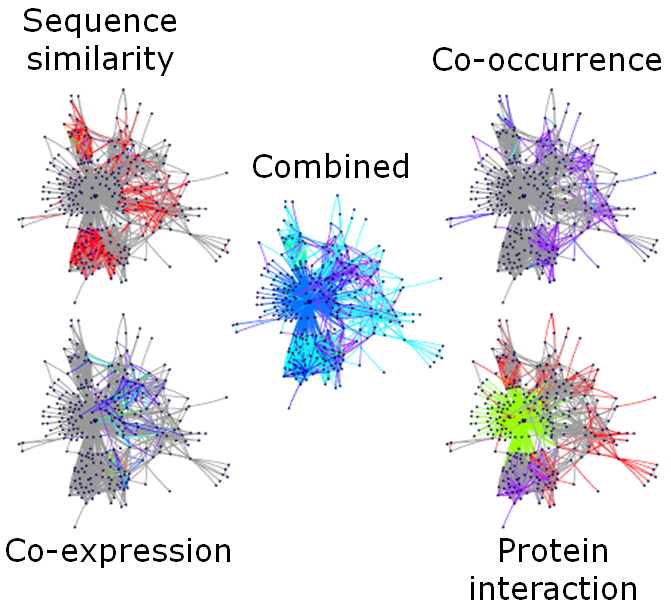
\includegraphics[scale=0.5]{images/Oct12/aba_cluster.png} 
\caption{Four sources of evidence on relations (+ all of them combined) using the rainbow scale colouring}
\label{fig:aba_cluster}
\end{figure}

Here are examples of combinations of steps, annotators and filters that can be used to analyse the data:
\begin{itemize}
\item Appearance -$>$ Layouts -$>$ Gem
\item Appearance -$>$ Smooth Relations to use anti-aliased painting (see Figure \ref{fig:aba_cluster_no_ann})

\begin{figure}[H]
\centering
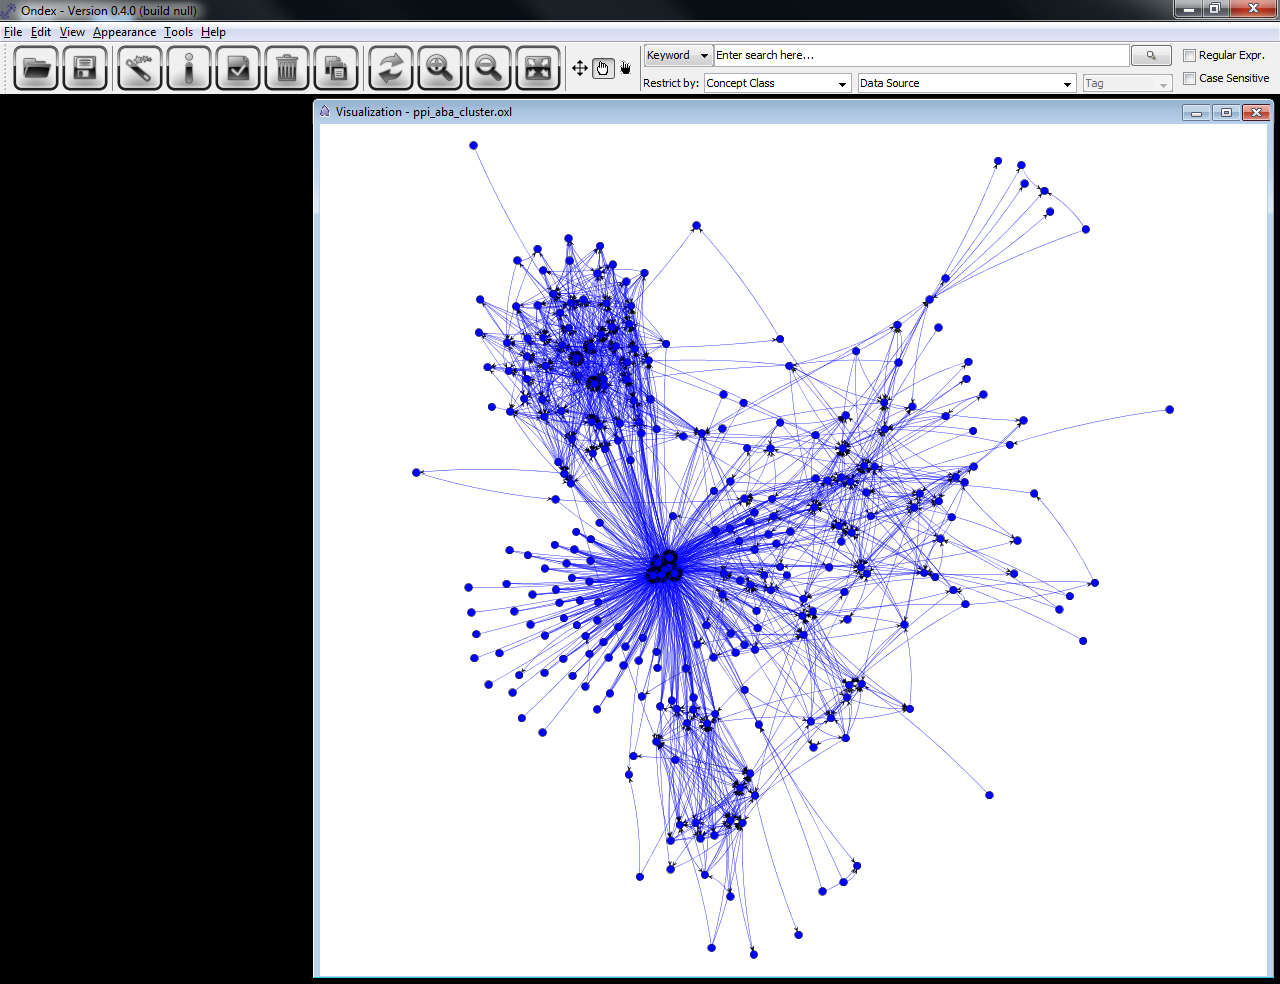
\includegraphics[scale=0.35]{images/Oct12/aba_cluster_no_ann.png} 
\caption{Abscisic acid cluster before annotation}
\label{fig:aba_cluster_no_ann}
\end{figure}

\item Tools -$>$ Annotators -$>$ Scale/Colour Relations by Numerical Value
\item Enter relation size of min 4 and max 4
\item Tick ``Colour relations'', ``No attribute colour'' and change colour to grey
\item Tick ``Colour on rainbow scale''
\item Select ``INTERACTION\_WEIGHT'' in list of attributes
\item Click on ``Annotate Graph'' (see results in Figure \ref{fig:aba_ann_rel})

\begin{figure}[H]
\centering
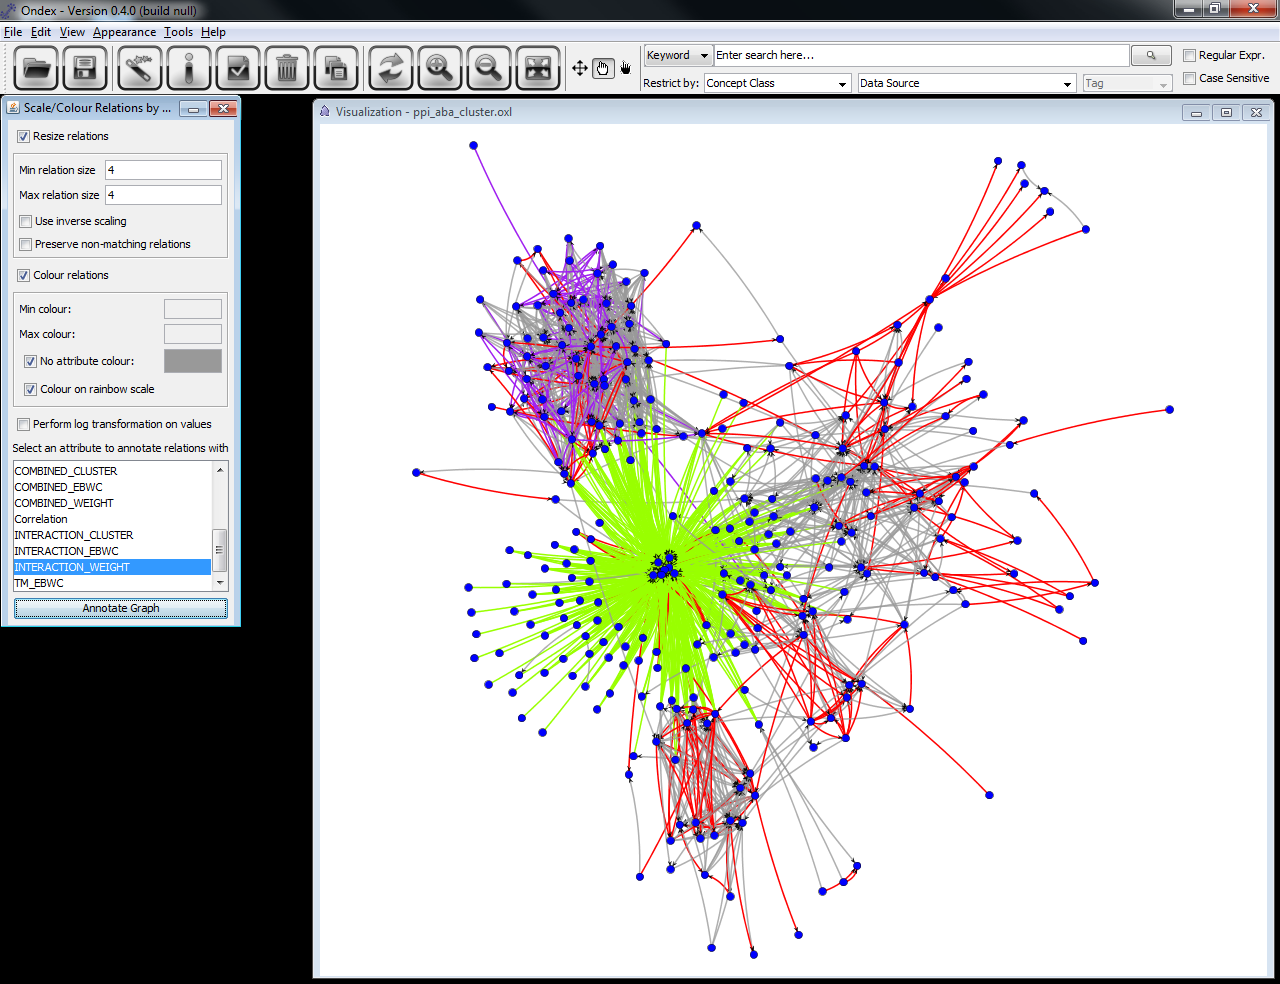
\includegraphics[scale=0.35]{images/Oct12/aba_ann_rel.png} 
\caption{Abscisic acid cluster after annotating relations}
\label{fig:aba_ann_rel}
\end{figure}

\item Tools -$>$ Annotators -$>$ Scale/Colour Concepts by Numerical Value
\item Enter concept size of min 10 and max 100
\item Tick ``No attribute size'' and enter 5
\item Tick ``Colour concepts''
\item Tick ``No attribute colour'' and select to grey
\item Tick ``Colour on rainbow scale''
\item Select ``COMBINED\_DC'' and click on ``Annotate Graph'' (see results in Figure \ref{fig:aba_ann_con})

\begin{figure}[H]
\centering
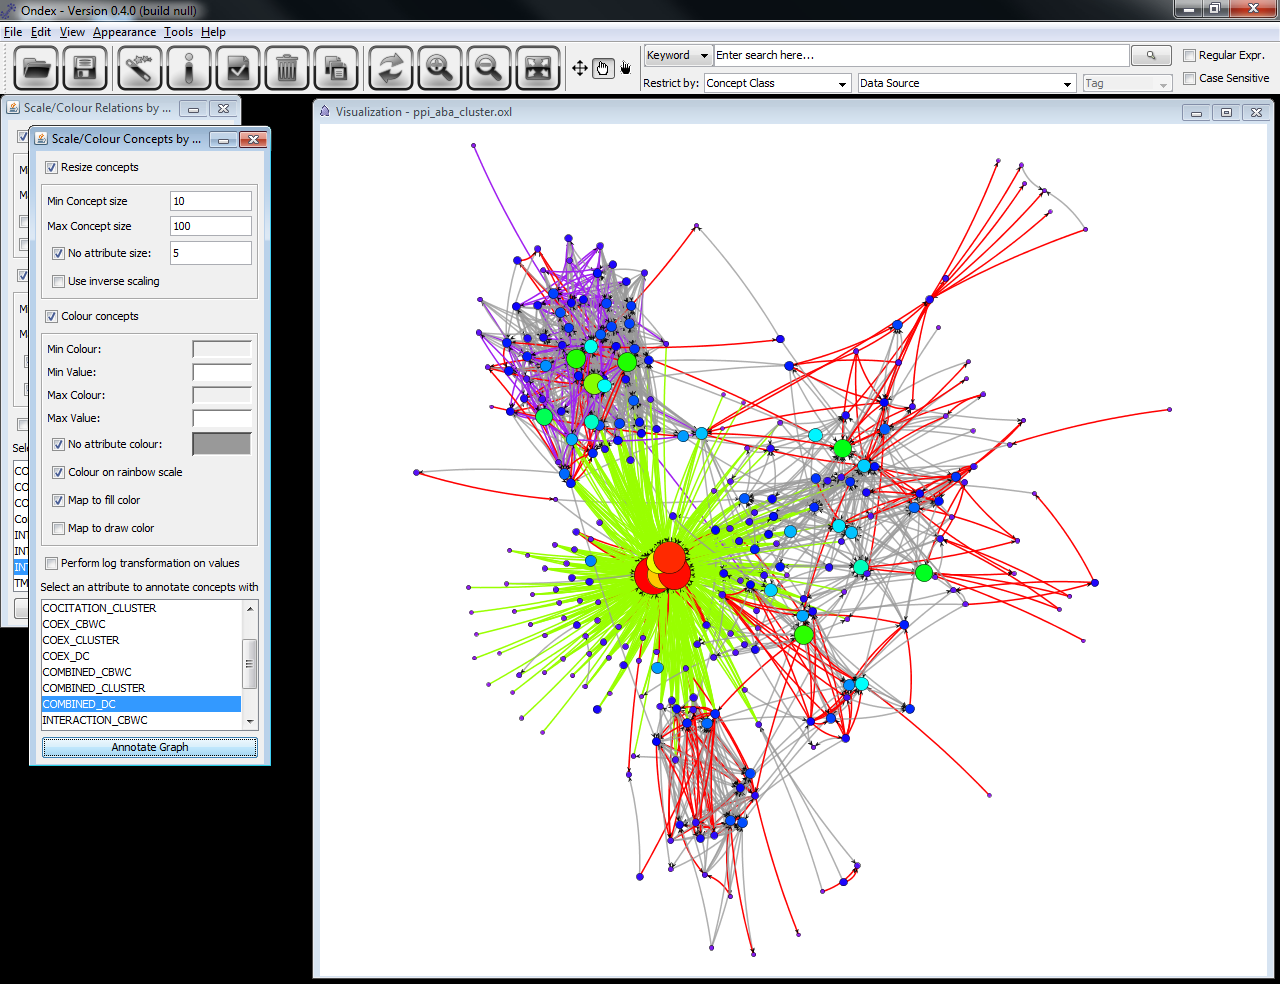
\includegraphics[scale=0.35]{images/Oct12/aba_ann_con.png} 
\caption{Abscisic acid cluster after annotating concepts}
\label{fig:aba_ann_con}
\end{figure}

\item Tools -$>$ Filters -$>$ More -$>$ Theshold	
\item Go to the ``Attributes on Relations'' tab
\item Select the ``INTERACTION\_EBWC'' (edge betweenness centrality) as attribute, a distribution should appear below (see Figure \ref{fig:aba_filter_thr1})

\begin{figure}[H]
\centering
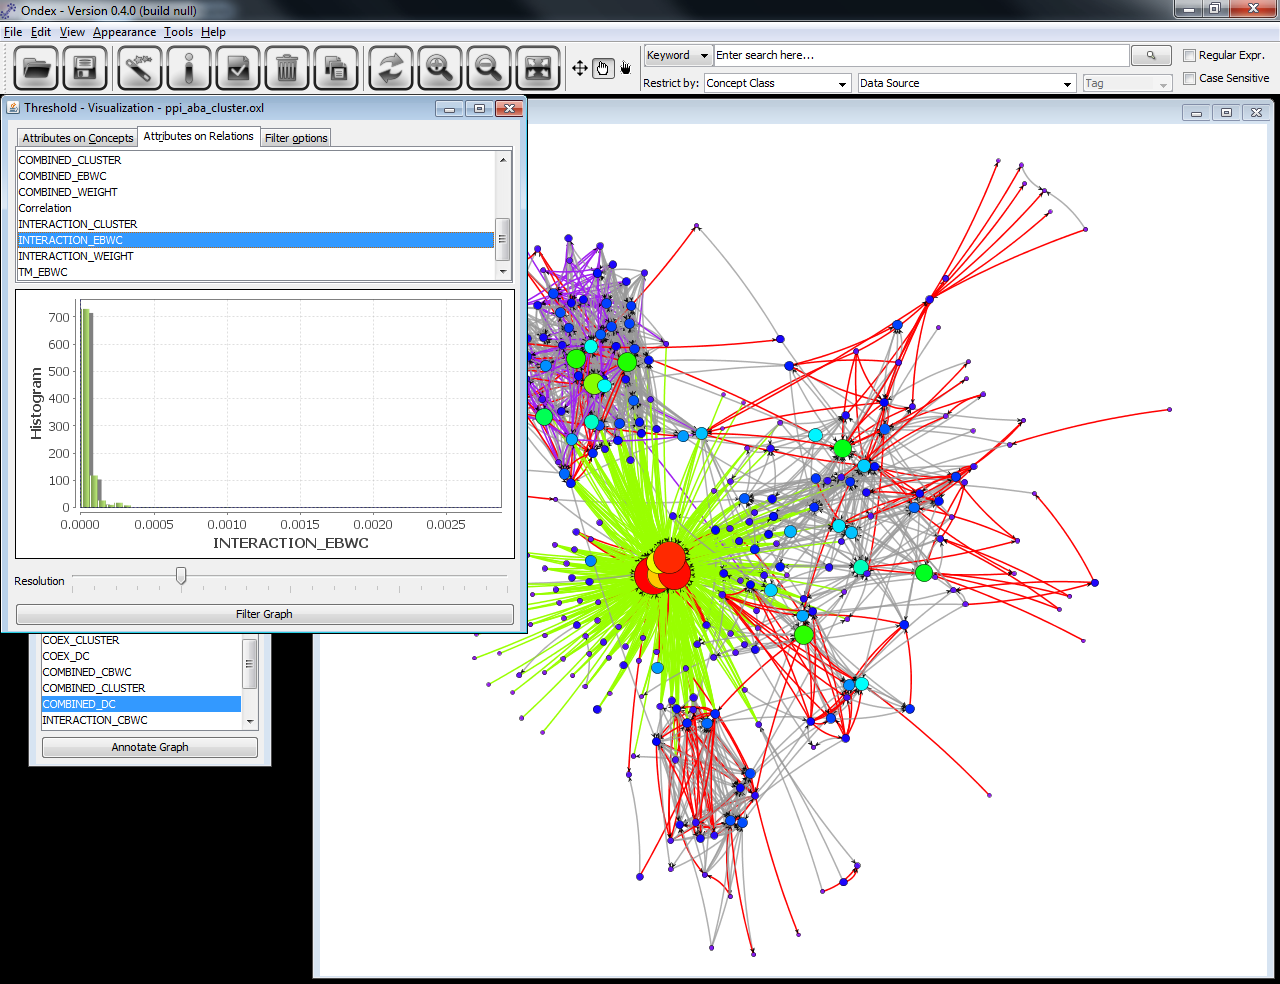
\includegraphics[scale=0.35]{images/Oct12/aba_filter_thr1.png} 
\caption{Before applying the Threshold filter}
\label{fig:aba_filter_thr1}
\end{figure}

\item Left-click to draw a rectangle to zoom in on the tail part of the distribution
\item Click anywhere in the distribution to select a threshold
\item Click on ``Filter Graph'' (see results in Figure \ref{fig:aba_filter_thr2}, some concepts/relations should disappear)

\begin{figure}[H]
\centering
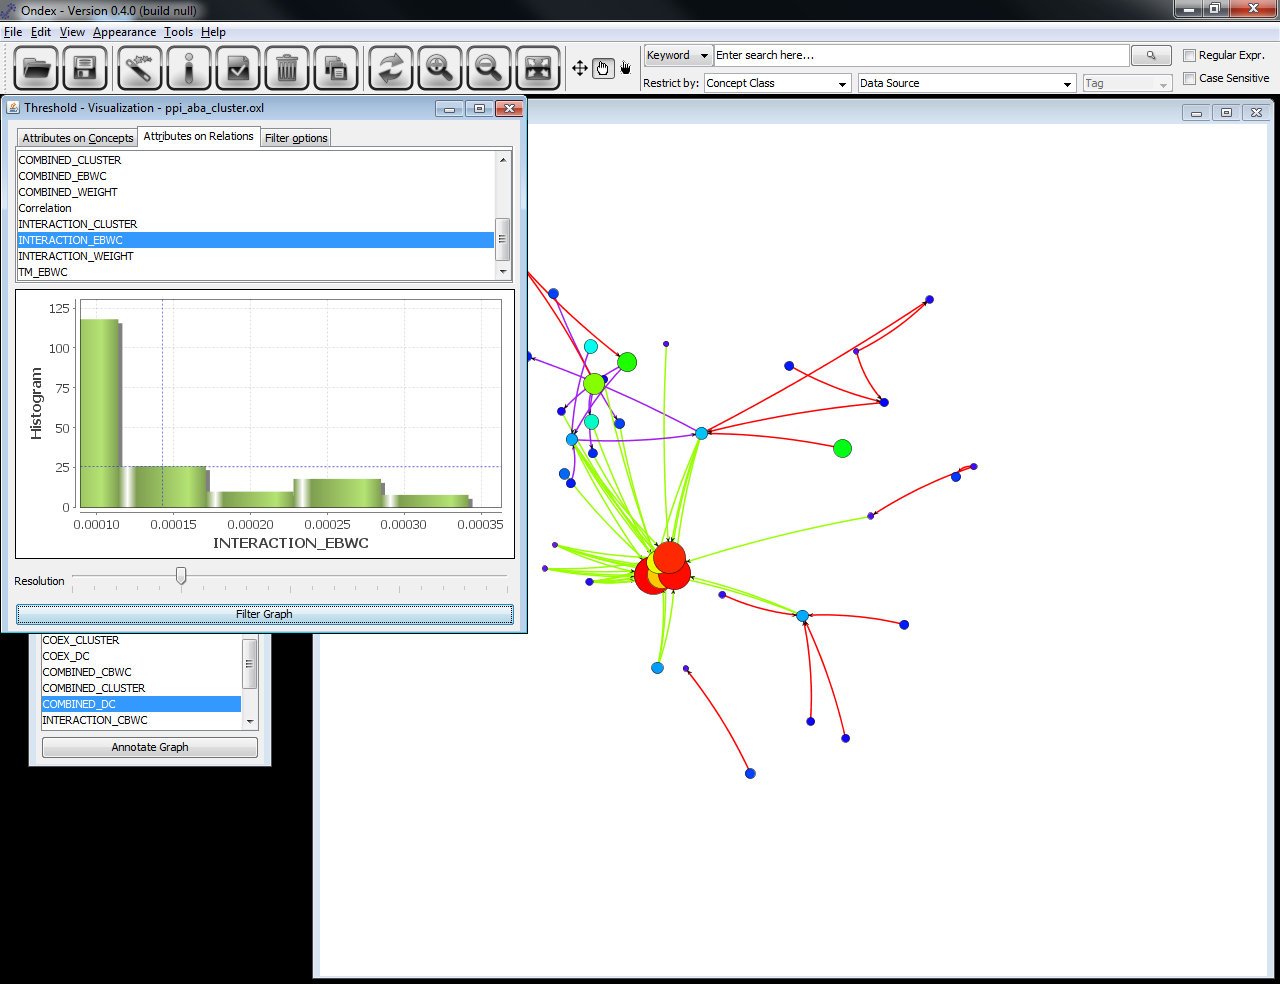
\includegraphics[scale=0.35]{images/Oct12/aba_filter_thr2.png} 
\caption{After zooming in on the distribution and applying the Threshold filter}
\label{fig:aba_filter_thr2}
\end{figure}

\item Appearance -$>$ Labels -$>$ Concepts
\item Zoom in and move concepts to look at the resulting PPI network (use shift and left-click to select a group of concepts to move)

\begin{figure}[H]
\centering
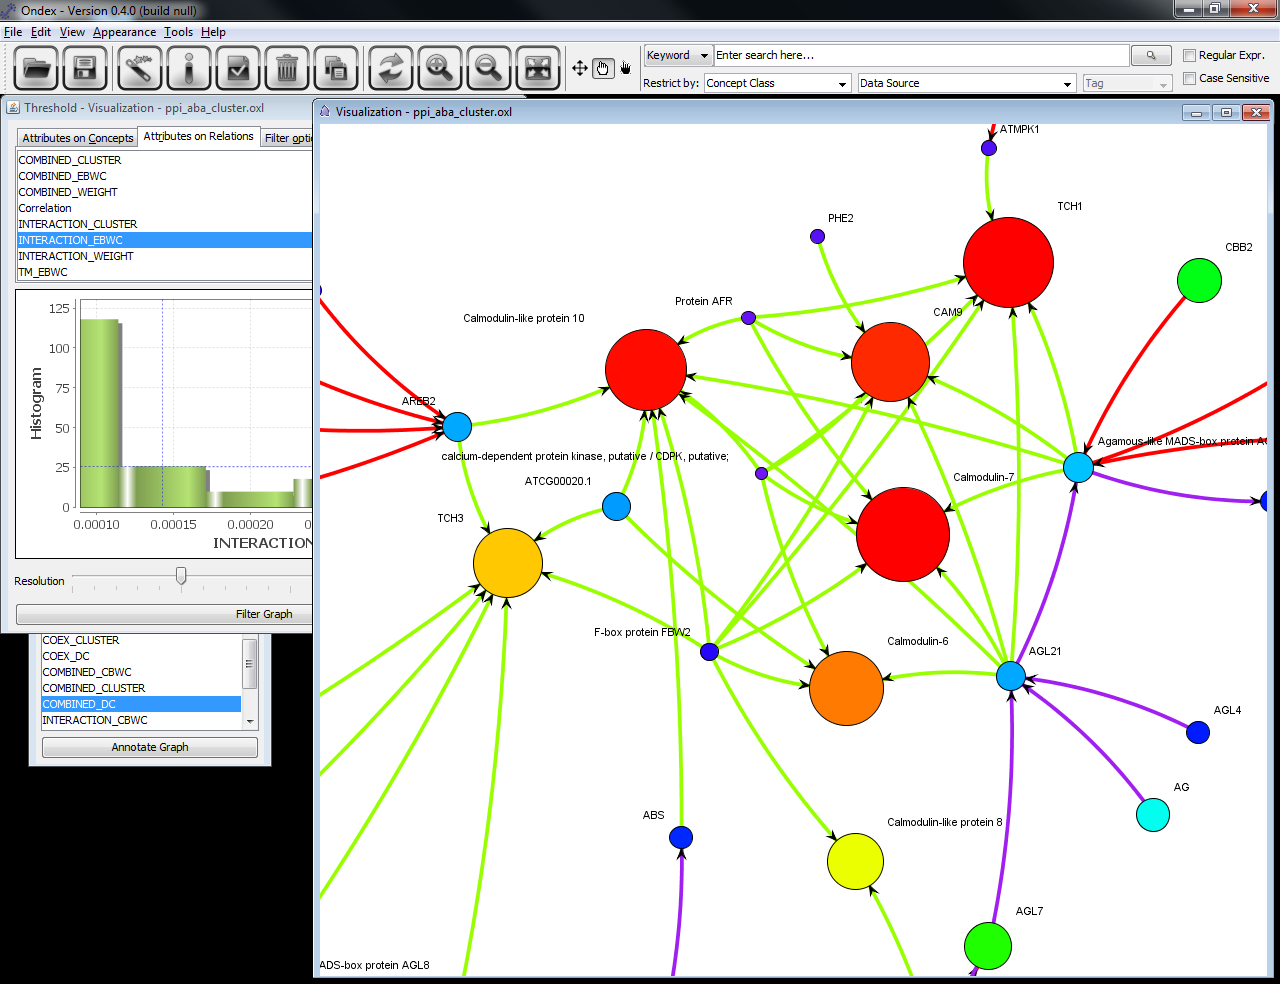
\includegraphics[scale=0.35]{images/Oct12/aba_cluster_annotated.png} 
\caption{After moving concepts to better reveal PPI}
\label{fig:aba_cluster_annotated}
\end{figure}

\end{itemize}

Experiment with the data and Ondex's tools to explore these \textit{Arabidopsis} protein-protein interactions further.
